\documentclass[12pt,a4paper,notitlepage,twoside]{report}

\usepackage{graphicx}
\usepackage{xcolor}
\usepackage[utf8]{inputenc} %unicode support
\usepackage[colorlinks=true]{hyperref}
\usepackage{enumitem}
\usepackage{tocbibind}
\usepackage[parfill]{parskip}
\usepackage[labelfont=bf]{caption}
\usepackage{fancyhdr}
%\usepackage[sf,compact]{titlesec}
\usepackage{listings}
\usepackage{geometry}
\usepackage{tikz}
\usepackage[subject={Comment},author={Rolf Huehne}, opacity=0.4,open=true]{pdfcomment}
\usepackage{soulutf8}

\geometry{top=1.0cm, left=2.4cm, right=0.6cm, bottom=1.0cm, includeheadfoot}

\renewcommand{\familydefault}{\sfdefault}

% Redefine the plain page style (used at chapter start)
\fancypagestyle{plain}{%
  \fancyhf{}%
\fancyfoot[LE]{\normalsize{\textbf{\thepage} \textbf{$\vert$}} \footnotesize{\textit{\leftmark}}}
\fancyfoot[RO]{\footnotesize{\textit{\leftmark}} \normalsize{\textbf{$\vert$} \textbf{\thepage}}}
  \renewcommand{\headrulewidth}{0pt}% Line at the header invisible
}

\pagestyle{fancy}
\fancyhf{}
\fancyhead[LE,RO]{\textit{\rightmark}}
\fancyhead[RE,LO]{\leftmark}
\fancyfoot[LE]{\normalsize{\textbf{\thepage} \textbf{$\vert$}} \footnotesize{\textit{\rightmark}}}
\fancyfoot[RO]{\footnotesize{\textit{\rightmark}} \normalsize{\textbf{$\vert$} \textbf{\thepage}}}

\setcounter{tocdepth}{3}
\setcounter{secnumdepth}{3}

\hyphenation{AgeFactDB JenAge JenAgeWiki HomoloGene PubMed Cytoscape BioLayout FMMM HTML life-span stand-alone}

\definecolor{afdb}{RGB}{255,100,25}
\definecolor{bglight}{RGB}{240,240,240}

\hypersetup{
  linkcolor=afdb
}

% Simplified hyperref referencing
%\newcommand{\rhref}{1}{in \autoref{#1} on \autopageref{#1}}

% PDF comments
\pdfcommentsetup{draft}
\definecolor{authorRH}{RGB}{255,100,25}
\definecolor{authorRHdark}{RGB}{255,83,0}
\definecolor{authorRHlight}{RGB}{255,196,142}

\defineavatar{RH}{author=Rolf,color=authorRH}

\newcommand{\pdfcRH}[2]{\pdfcomment[avatar=RH #1]{#2}}
\newcommand{\pdfmhRH}[3]{\pdfcomment[avatar=RH #1]{#2} \sethlcolor{authorRHlight} \hl{#3}}
\newcommand{\pdfmsRH}[3]{\pdfcomment[avatar=RH #1]{#2} \setstcolor{authorRH} \st{#3}}
\newcommand{\pdfmuRH}[3]{\pdfcomment[avatar=RH #1]{#2} \setulcolor{authorRH} \ul{#3}}

%\newcommand{\pdfmhRH}[3]{\pdfcomment[avatar=RH #1]{#2} \sethlcolor{authorRHlight} }
%\newcommand{\pdfmsRH}[3]{\pdfcomment[avatar=RH #1]{#2} \setstcolor{authorRH} }


\setlist{noitemsep}

%%% Begin ...
\begin{document}

\title{AgeFactDB Documentation}
\author{Rolf H\"{u}hne}
%\maketitle

\begin{titlepage}
	\centering
	{\huge\bfseries JANet - \underline{J}mol \underline{A}geFactDB \underline{Net}work-viewer\par}
	\vspace{1cm}
	{\huge\bfseries Documentation\par}
	\vspace{1cm}
	{\Large\itshape by Rolf H\"{u}hne\par}
	\vfill

	\vfill

% Bottom of the page
	{\large \today\par}
\end{titlepage}

\tableofcontents
\listoffigures

\chapter{Introduction}
\label{chap:introduction}



\chapter{Background}
\label{chap:background}

\section{AgeFactDB}
\label{sec:agefactdb}

\subsection{Description}
"AgeFactDB (\href{http://agefactdb.jenage.de}{http://agefactdb.jenage.de}) is a database aimed at the collection and integration of ageing phenotype data including lifespan information. Ageing factors are considered to be genes, chemical compounds or other factors such as dietary restriction, whose action results in a changed lifespan or another ageing phenotype. Any information related to the effects of ageing factors is called an observation and is presented on observation pages. To provide concise access to the complete information for a particular ageing factor, corresponding observations are also summarized on ageing factor pages. In a first step, ageing-related data were primarily taken from existing databases such as the Ageing Gene Database--GenAge, the Lifespan Observations Database and the Dietary Restriction Gene Database--GenDR. In addition, it was started to include new ageing-related information. Based on homology data taken from the HomoloGene Database, AgeFactDB also provides observation and ageing factor pages of genes that are homologous to known ageing-related genes. These homologues are considered as candidate or putative ageing-related genes." \cite{huehne2014}

\subsection{Ageing Factors}
Currently there are implemented three types of ageing factors:
\begin{enumerate}[label=\textbf{\arabic*.}]
\item Gene
\item Compound
\item Other Ageing Factor
\end{enumerate}

\subsubsection{Genes}
If available, the NCBI Gene ID is used for the identification of genes, to avoid duplicate entries with different names.

If it is not provided, it is tried to assign it automatically using the synonym database GPSDB  and the NCBI Gene database. If multiple NCBI Gene IDs might match, no NCBI Gene ID is assigned and only gene symbol and species are used for the integration.

Internally always gene symbol, species, and NCBI Gene ID are used to identify a gene. Depending on the information provided by the data source, GPSDB, and NCBI Gene it is possible that the same gene symbol/species combination is included multiple times into AgeFactDB, with and without one or more different NCBI Gene IDs.

\subsubsection{Compounds}
Chemical compounds are currently identified by the name who was used in the AgeFactDB source databases. No synonym information is used yet within AgeFactDB.

\subsubsection{Other Ageing Factors}
Other ageing factors are for example dietary restriction and heat shock.

Similar to chemical compounds they are currently only identified by their name. Because it is difficult to judge the slight differences that might be involved for example between 'dietary restriction' and 'caloric restriction', it wasn't done any unification yet.

\subsection{Putative Ageing Factors}
\label{sec:putative_ageing_factors}
In addition to genes with experimental ageing relevance evidence, AgeFactDB includes also genes homologous to these genes as putative ageing factors. They are identified by a homology analysis based on the HomoloGene database from the NCBI.

In contrast to other ageing-related databases, where homologous genes are just named inside a gene page, they are included in the same way as the genes with experimental ageing relevance evidence. This way the full features are also available for the putative ageing factors. 

Ageing factors are discriminated from putative ageing factors inside the AgeFactDB web interface by a color coding system shown in Figure \ref{fig:ageing_relevance_evidence} on page \pageref{fig:ageing_relevance_evidence}. Green indicates experimental evidence with an effect on ageing, red indicates experimental evidence with no effect on ageing, and blue indicates computational ageing relevance evidence. The color of all observations assigned to an ageing factor determine the color of the ageing factor, with the following priority:  green, red, blue. In addition to the major color all other assigned colors are also indicated as small squares.

 \begin{figure*}[!ht]
      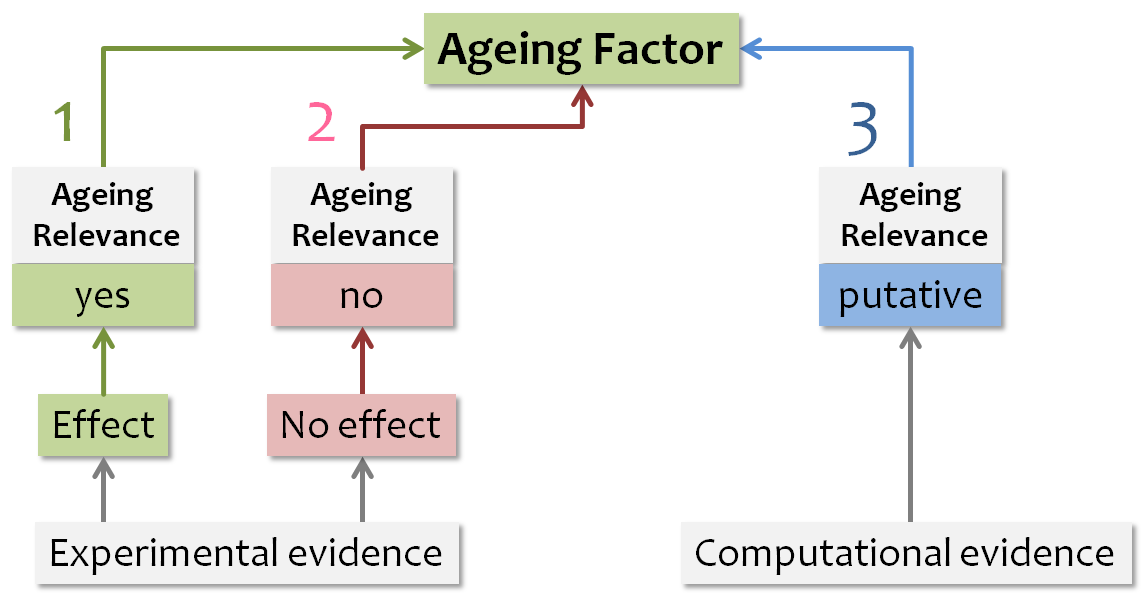
\includegraphics[width=0.96\textwidth]{data/ageing_relevance_evidence.png}
  \caption[Ageing Relevance Evidence Color Codes]{Ageing Relevance Evidence Color Codes. 
  \newline \textit{Color coding system to indicate the type of ageing relevance evidence available for ageing factors. The priority for assigning a color to the ageing factor is indicated by the number: 1 has highest priority, 3 has lowest priority.}
      \label{fig:ageing_relevance_evidence}
      }
\end{figure*}


\subsection{Observations}
Currently there are implemented three types of observations:
\begin{enumerate}[label=\textbf{\arabic*.}]
\item Ageing Phenotype Data Type 1 (phenotype\_1)
\item Ageing Phenotype Data Type 2 (phenotype\_2)
\item Homology Analysis (homology\_analysis)
\end{enumerate}

The names in brackets are the internal names filled into table fields, the others are the 'official' names used in the web interface. Initially, the first two types were named 'phenotype' and 'lifespan'. But this didn't really fit, because lifespan is also a phenotype and because some phenotype observations also contained lifespan data. So it was switched to a technical distinction. 'Data type 1' are free-text ageing phenotype observations and 'data type 2' are structured ageing phenotype observations, while 'Homology analysis' observations are structured computational observations. But the table names still follow the original naming scheme (lifespan, phenotype).

\subsection{Unification}
\label{sec:unification}
The same genes might have been integrated into two different source databases or even the same source database with different names.  

It was tried to resolve this by using the gene/protein synonym database GPSDB and integrate the gene into AgeFactDB using the name marked as preferred name in GPSDB.

All name changes are listed in a table within the \href{http://agefactdb.jenage.de/cgi-bin/jaDB.cgi?VIEW=release}{release page}, shown partially in Figure \ref{fig:name_changes} on page \pageref{fig:name_changes}.

 \begin{figure*}[!ht]
      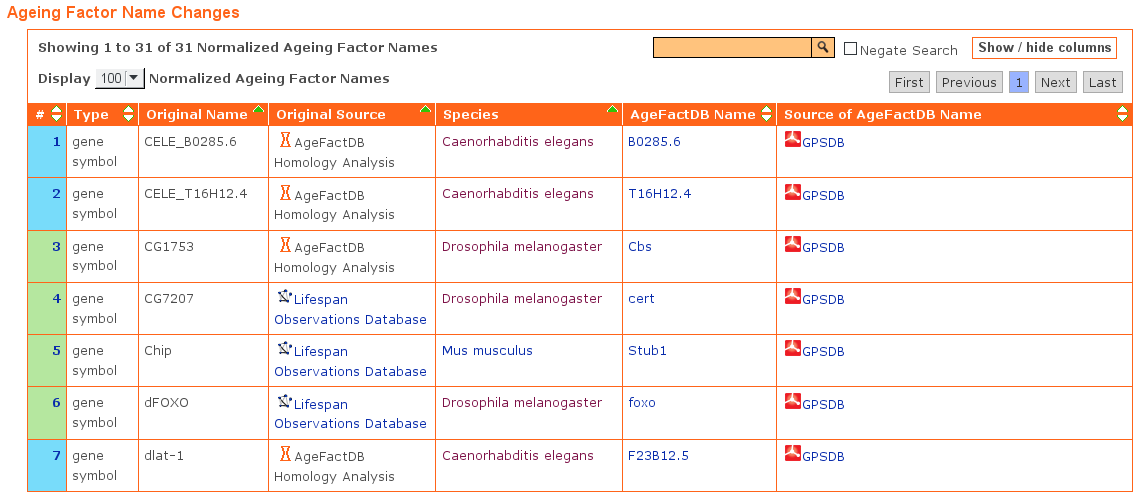
\includegraphics[width=0.96\textwidth]{data/name_changes.png}
  \caption[Ageing Factor Name Changes]{Ageing Factor Name Changes. 
  \newline \textit{Partial list of the ageing factor name changes as a result of the unification.}
      \label{fig:name_changes}
      }
\end{figure*}




%\cleardoublepage
%\phantomsection
%\addcontentsline{toc}{chapter}{Bibliography}
\bibliographystyle{abbrv}
\bibliography{janet-documentation}      % Bibliography file (usually '*.bib' )

\end{document}
